De relevante oplysninger vi har fået at vide om lufthavnens trafik er:
\begin{itemize}
\item Der ankommer i gennemsnit $200$ fly om dagen, men på en given dag kan der både ankomme færre eller flere.
\item Trafikken ankommer indenfor en periode på $13$ timer. 
\item Ankomsttidspunkterne er tilfældige inden for perioden og ikke koordineret flyene imellem. 
\item Trafikken forventes at stige med $5\%$ om året fremover. 
\end{itemize}
Et sådant setup er klassisk indenfor modellering af systemer hvor begivenheder sker tilfældigt i tid. Lignende eksempler kunne være ankomst af opgaver til en computerserver, kø på apoteket, tidspunkter for jordskælv, ulykker på motervej og henfald af radioaktive partikler. Alle disse eksempler kalder man for \textit{punktprocesser} hvor tidsperioden mellem to hændelser er tilfældige variable $T_1, T_2,\dots$ som illustreret i figur \ref{fig:process1}. 
\begin{figure}
\centering
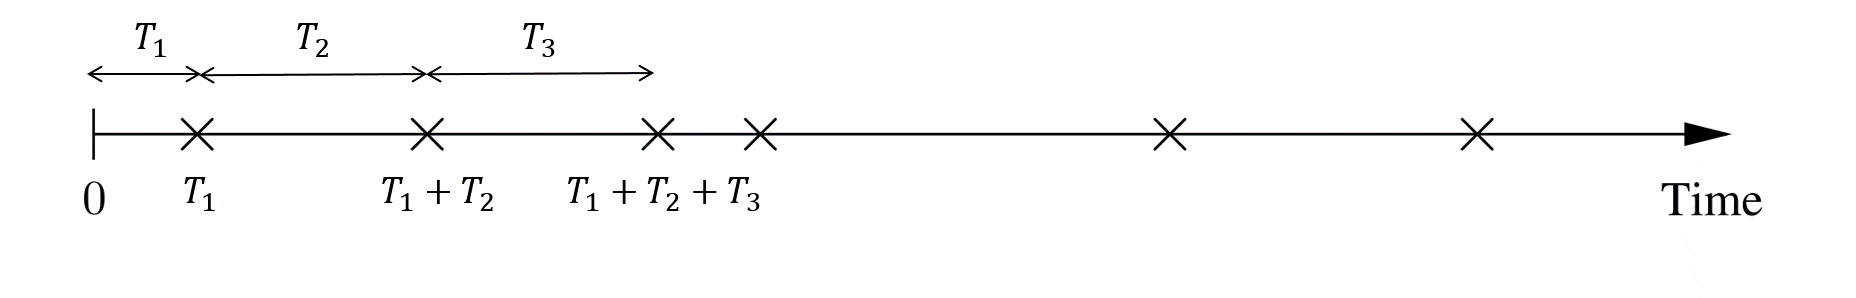
\includegraphics[width = \textwidth]{process1.png}
\caption{Punktprocess hvor $\times$ markerer hændelser i tid - eksempelvis ankomsttidspunkter af fly.} \label{fig:process1}
\end{figure}
Det viser sig, at når man antager uafhængighed mellem tidspunkter\footnote{Se \cite[123-127]{olofsson2012} for de præcise detaljer.}, da vil $T_1, T_2,\dots$ nødvendigvis følge en såkaldt \textit{eksponentielfordeling} med rate $\lambda$ og vi kalder punktprocessen for en \textit{Poisson process}. \\
En exponentielfordeling er en kontinuert fordeling og hvis $X$ følger en eksponentielfordeling med rate $\lambda$ da er pdf funktionen\footnote{Man kan simulere tal fra eksponentielfordelingen med \texttt{numpy.random.exponential} hvor man skal angive parametret \texttt{scale}. \texttt{scale} svarer til $\lambda^{-1}$}:
\begin{align*}
p_X(x) = \lambda e^{-\lambda x}, \quad x \geq 0,
\end{align*}
og vi skriver $X \sim \exp(\lambda)$ (se figur \ref{fig:distributions}). Raten $\lambda$ i eksponentielfordelingen har indflydelse på hvor hurtigt vi ser et udfald og en eksponentialtfordelt $X$ vil i gennemsnit have udfaldet $1/\lambda$. I en Poisson fordeling har vi altså at $T_i \sim \exp(\lambda)$ for $i = 1,2\dots,$ hvor hver $T_i$ har gennemsnit $1/\lambda$.
\\ \\
Følgende resultat om Possion processer er nyttigt. Lad $X(t)$ være en tilfældig variabel der tæller antallet af punkter fra $0$ til $t$ i en Poisson process med rate $\lambda$. Det viser sig da at $X(t)$ følger den såkaldte \textit{Possion fordeling} med parameteren $k = \lambda t$. En Poisson fordeling er en diskret fordeling og hvis $X$ følger en Poisson fordeling med parameter $k$ da er pmf funktionen\footnote{Man kan simulere tal fra Poissonfordelingen med \texttt{np.random.poisson} hvor man skal angive parameteret \texttt{lamb}. \texttt{lamb} svarer til $k$.}
\begin{align*}
p_X(x) = e^{-k}\frac{k^x}{x!}, \quad x = 0,1,\dots
\end{align*}

\begin{figure}
\centering
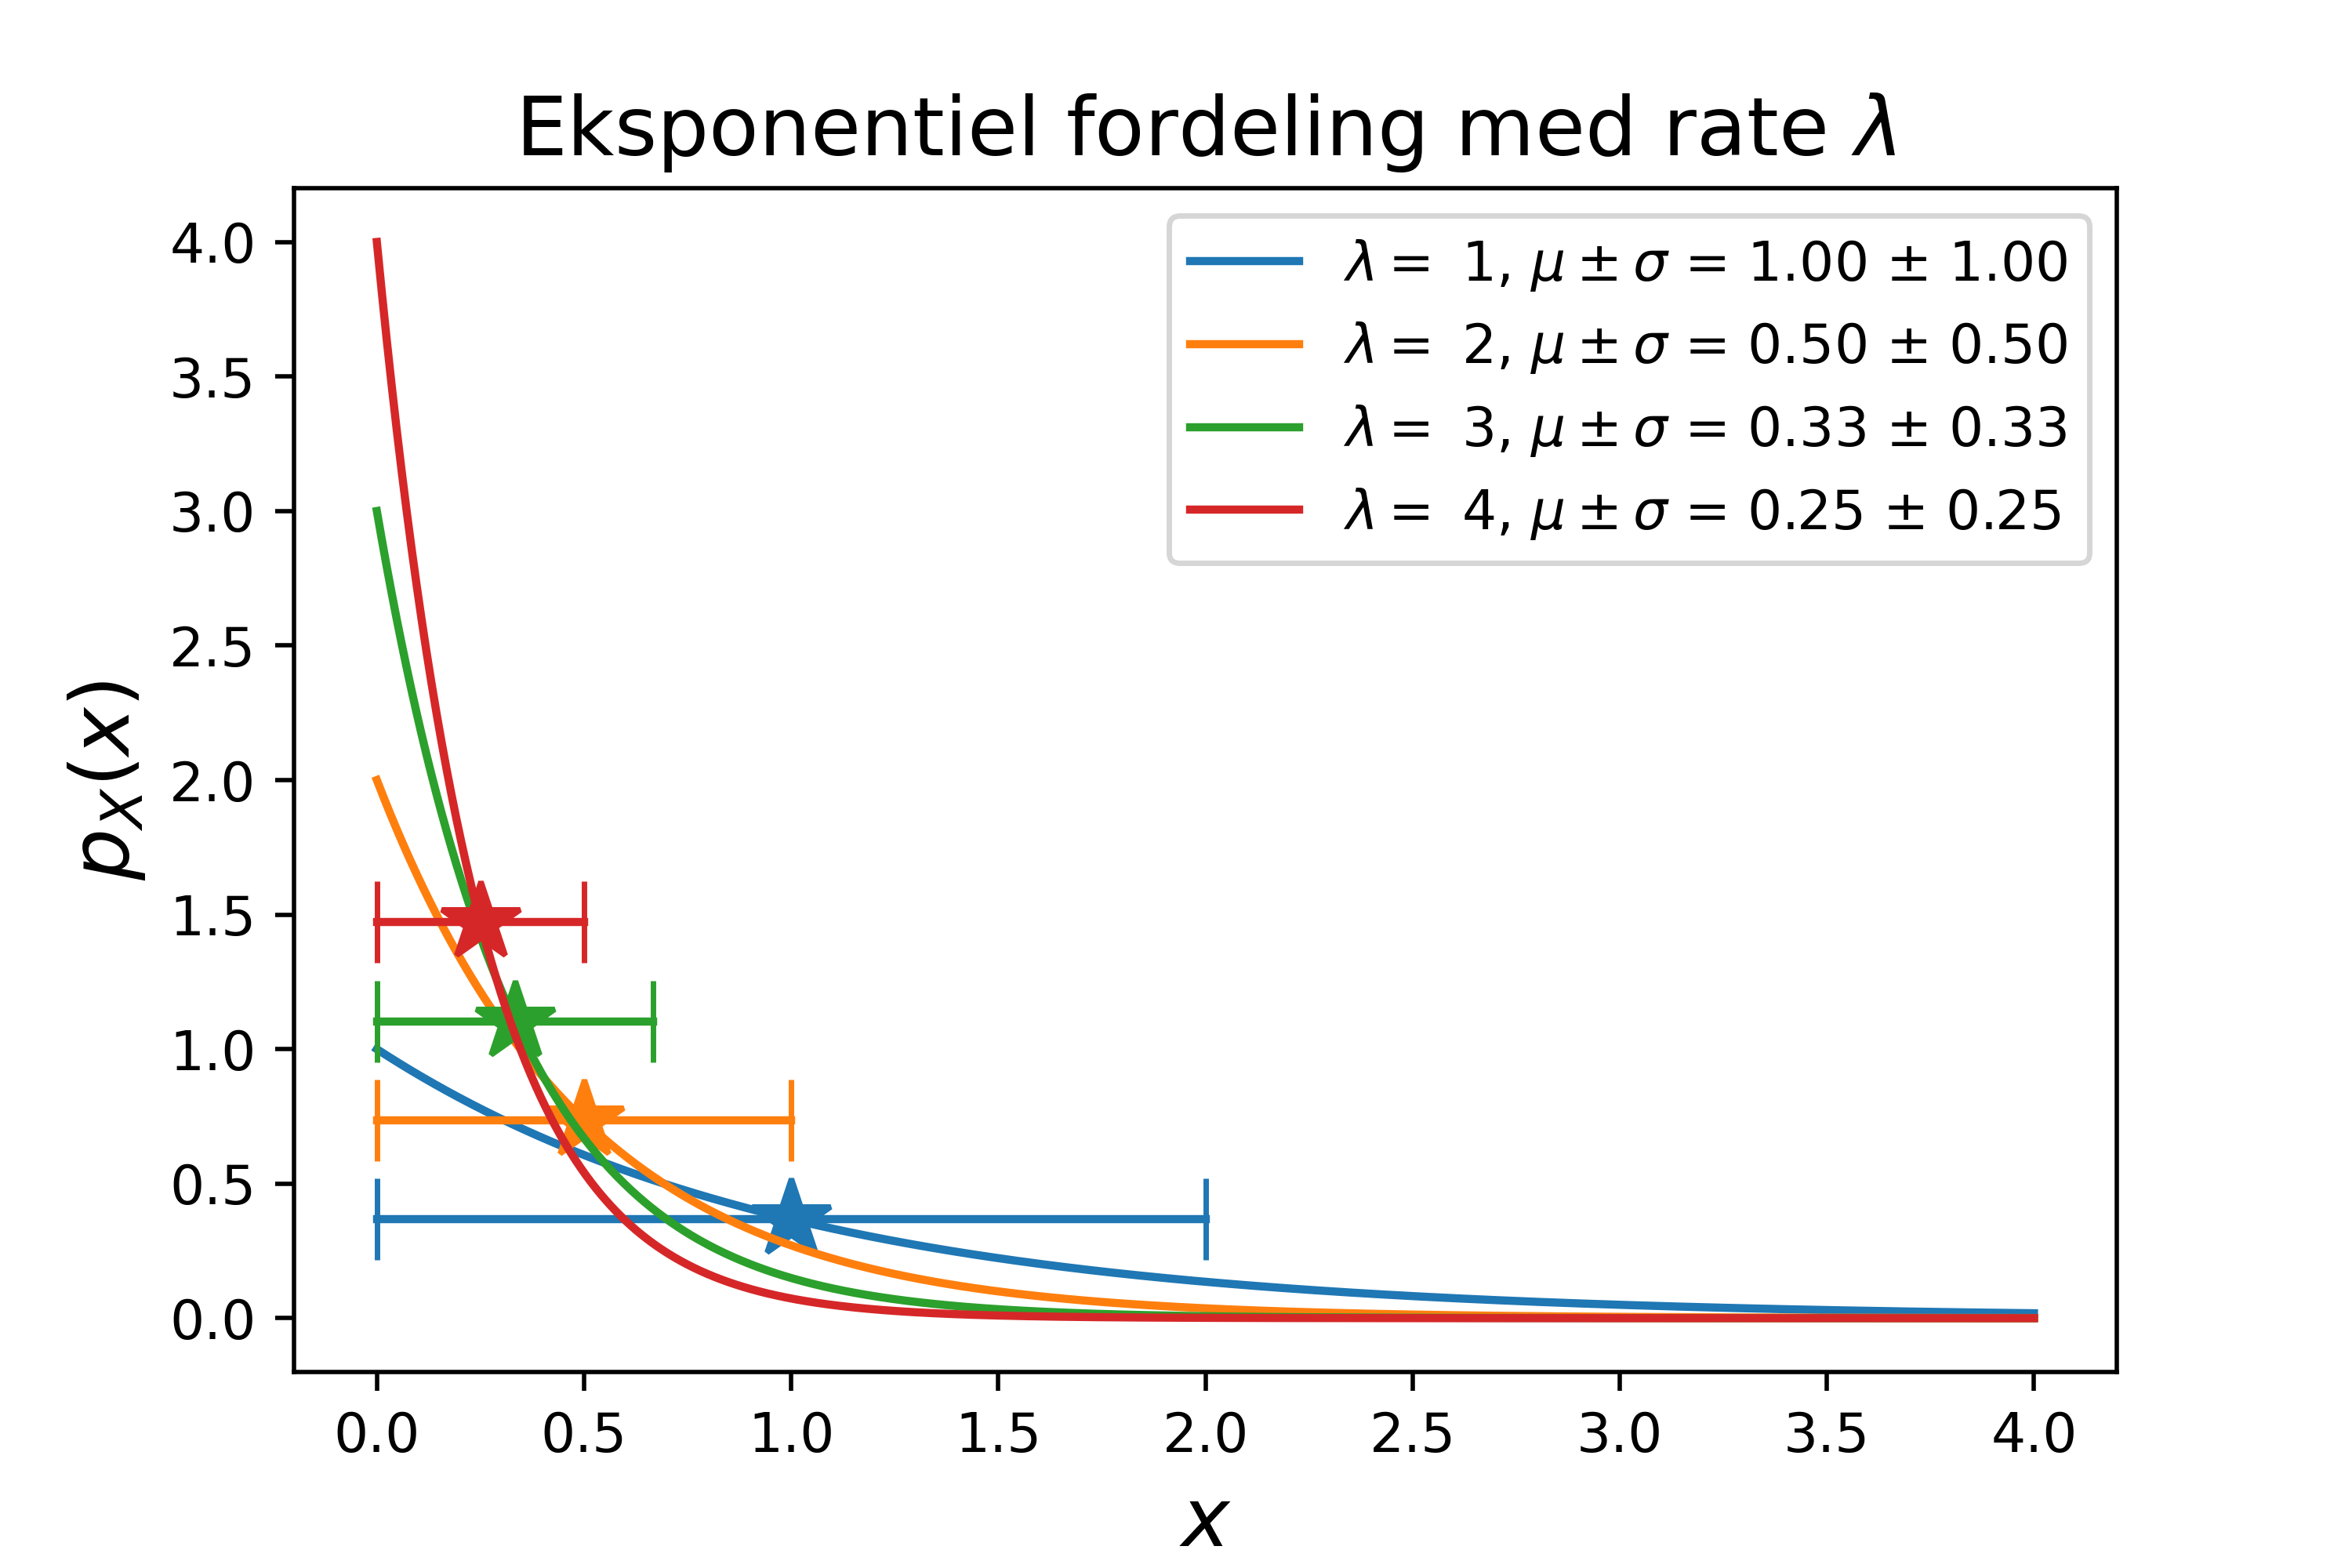
\includegraphics[width = 0.45\textwidth]{exp_dist.png}
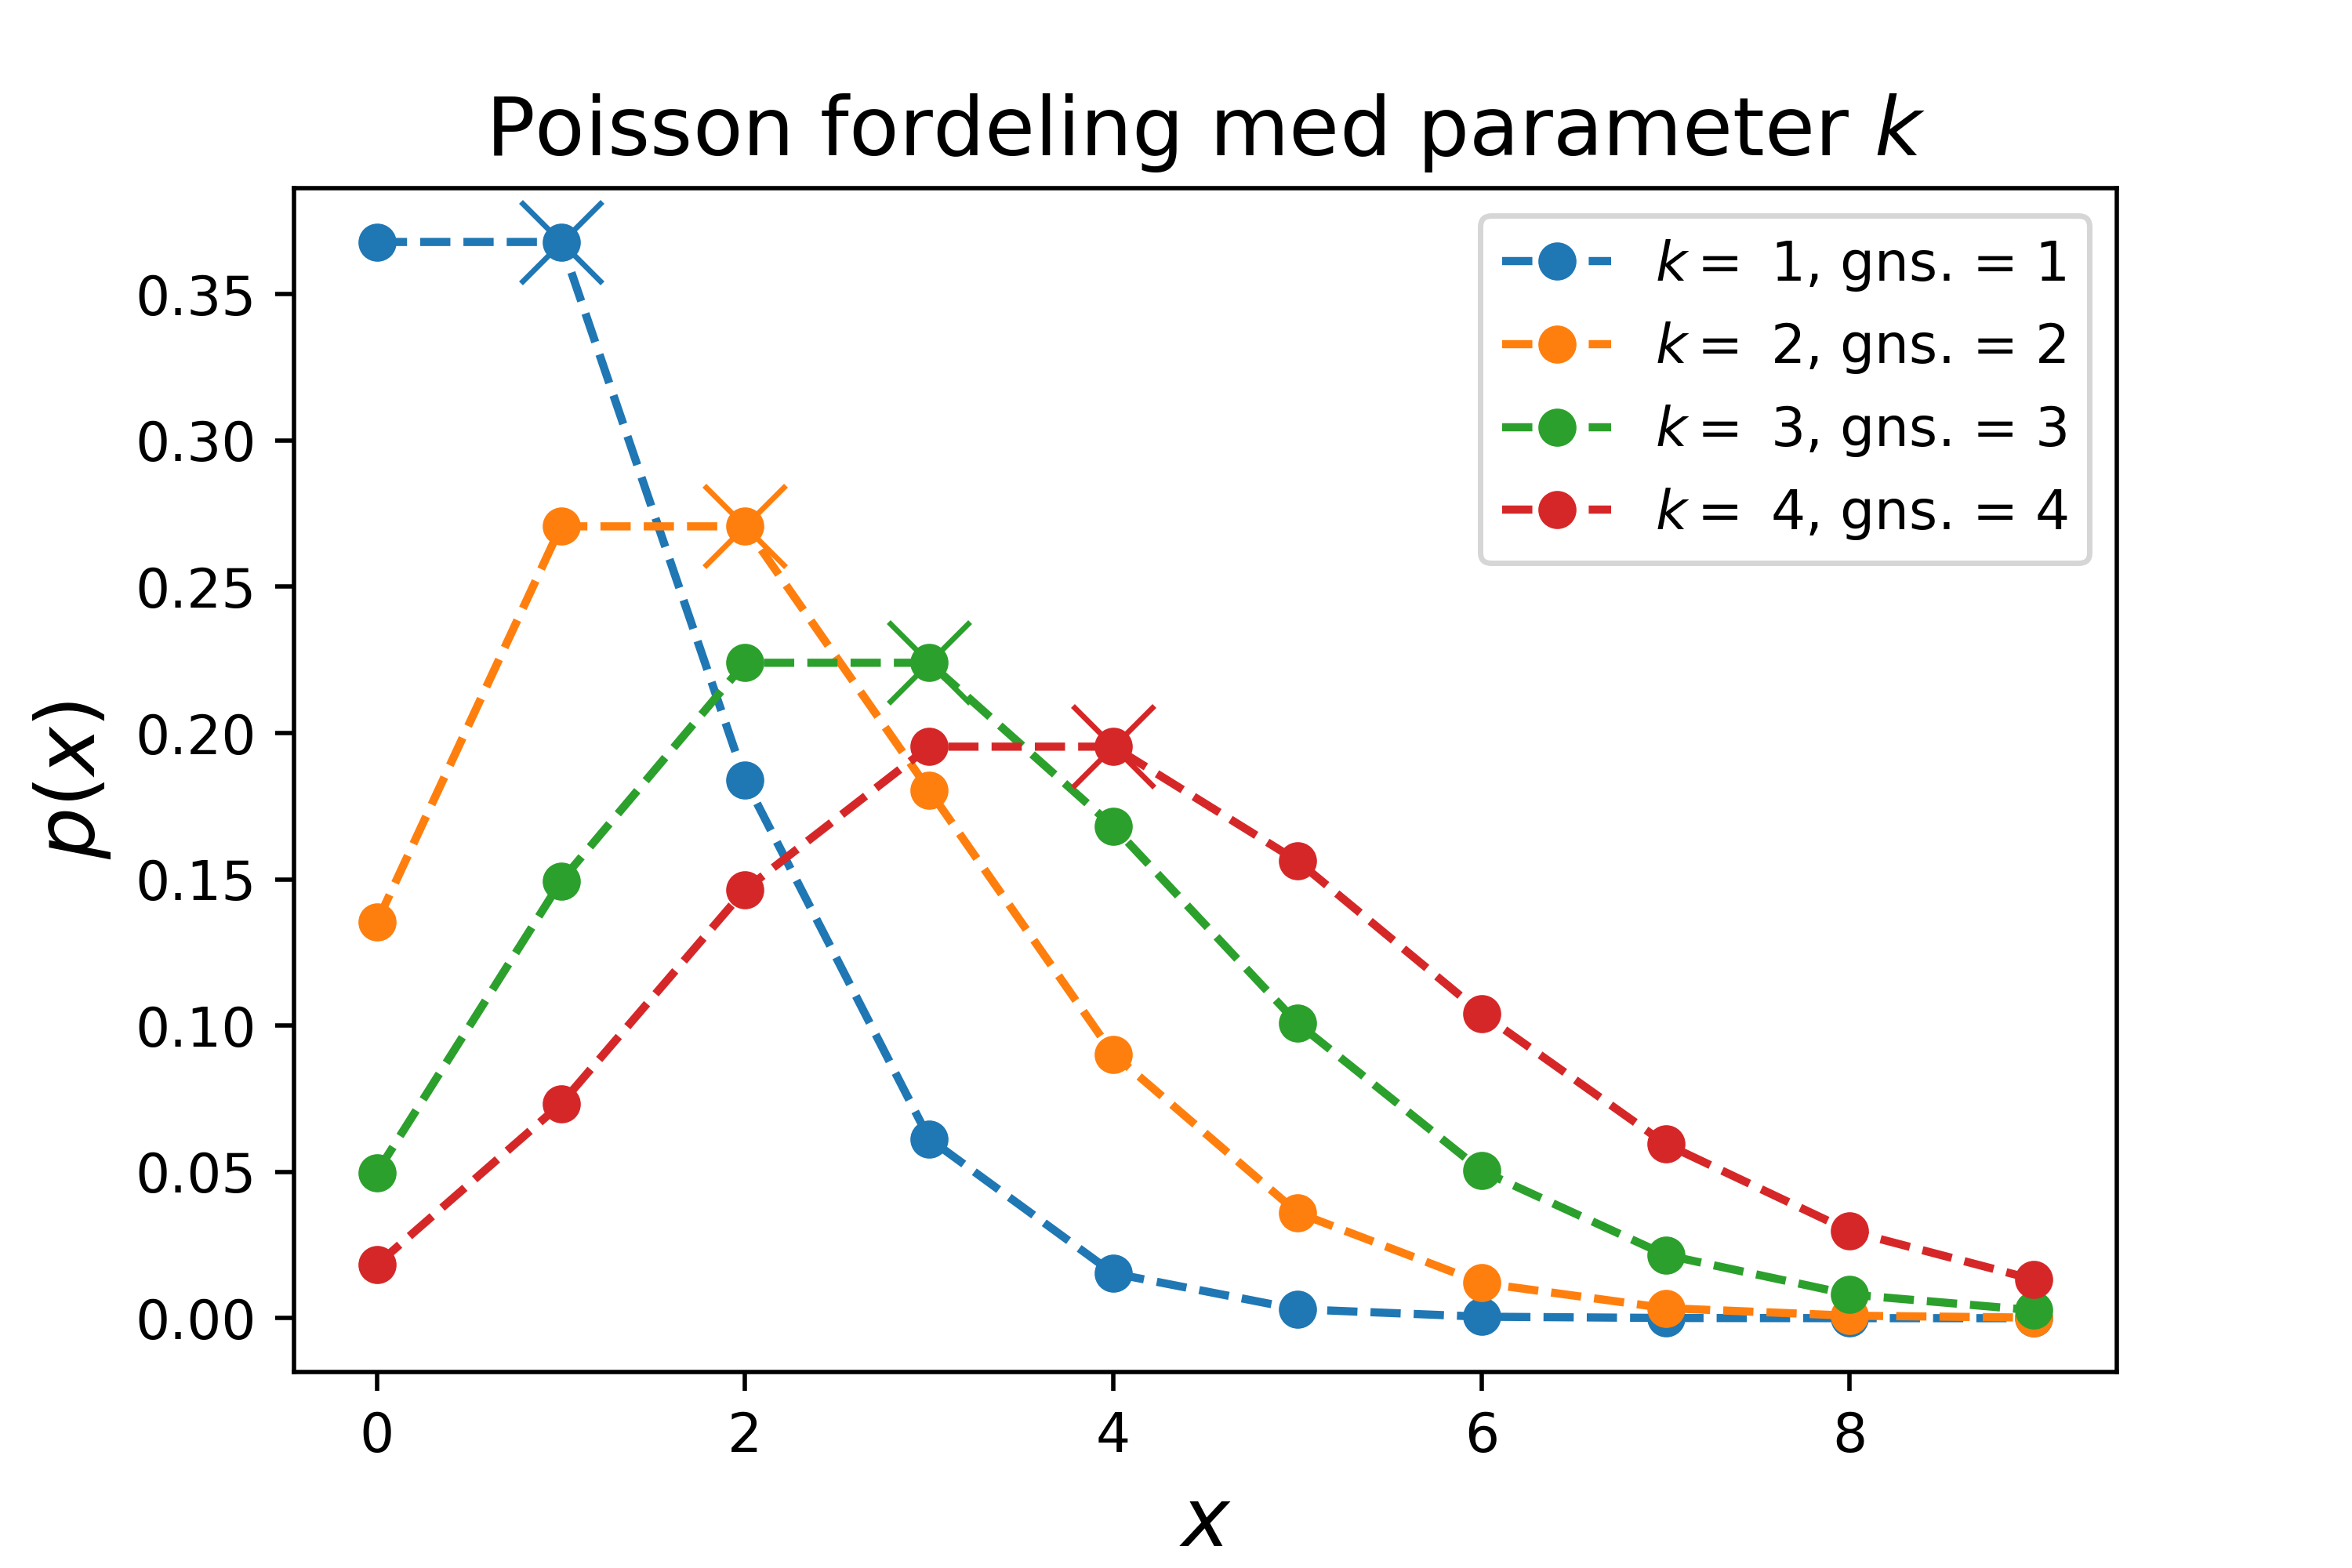
\includegraphics[width = 0.45\textwidth]{poiss_dist.png}
\caption{pdf og pmf for eksponentiel og Poisson fordeling. $\times$ markerer gennemsnit ved de forskellige parametre.} \label{fig:distributions}
\end{figure}
Den gennemsnitlige værdi af en Poisson fordeling med parameter $k$ er blot $k$ (se figur \ref{fig:distributions}). Lad os se på følgende eksempel: En Possson process har rate $\lambda = 2$. Ud fra resultatet vil antal punkter ved $t = 10$ sekunder være Poisson fordelt med parameter $k = 20$ og vi forventer gennemsnitligt $20$ punkter ved $t = 10$. 
\\ \\
Et sidste nyttigt resultat kan bruges til nemt at simulere en Poisson process. Vi har givet en Poisson process med rate $\lambda$. Givet at der er $N$ antal punkter i tidsperioden $[0,t]$ vil fordelingen for tidspunkterne være uafhængigt uniformt fordelte tilfældige variable i intervallet $[0,t]$. Kender vi $N$ kan man altså blot simulere $N$ punkter uniformt fordelt i intervallet $[0,t]$ for at simulere en Poisson process.
\\ \\
I kan læse mere om eksponentielfordelinger, Poissonfordelinger og Poisson processer i \cite{olofsson2012} (online version er gratis tilgængelig på AUB). Heri finder i også beviser for resultaterne om Poisson processen. Ovenstående er dog til tilstrækkeligt til at generere de tal vi skal bruge i miniprojektet. Overvej følgende spørgsmål for at simulere ankomsttidspunkter af fly: 
\begin{itemize}
\item Hvordan kan man bestemme rate parametren $\lambda$ ud fra de givne oplysninger? 
\item Hvordan kan man simulere antal fly på en dag?
\item Hvordan kan man simulere ankomsttidspunkter givet antal fly på en dag?  
\item Hvordan kan effekten af stigende trafik på $5\%$ om året simuleres? Hint: Brug $\lambda$. 
\end{itemize}